\documentclass[a4paper]{article}
\usepackage[14pt]{extsizes}
\usepackage[utf8]{inputenc}

\usepackage[russian]{babel}
\addto\captionsrussian{\renewcommand{\figurename}{Рисунок}}

\usepackage{caption}
\captionsetup{justification = raggedright,
	          singlelinecheck = false,
              font = {small, it}}

\usepackage[left=20mm, top=15mm, right=15mm, bottom=15mm, nohead, footskip=10mm]{geometry}

\usepackage{amsmath}

\usepackage{graphicx}
\graphicspath{{./images/}}
\DeclareGraphicsExtensions{.png}

\usepackage{adjustbox, array}

\usepackage{dcolumn}
\newcolumntype{M}[1]{>{\centering\arraybackslash}m{#1}}

\usepackage{titlesec}
\titleformat{\section}{\normalfont\fontsize{18}{0pt}\bfseries}{\thesection}{}{}

\usepackage{setspace}

\usepackage{enumitem}
\setlist{nolistsep, topsep=8pt, parsep=3pt, leftmargin=1.5cm}

\renewcommand{\labelitemi}{$ \circ $\hspace{0.225em}}

\begin{document}
	
	\begin{center}
		
		\  \vskip 10cm
		
		\fontsize{20}{16pt} \selectfont {Лабораторная работа № 6: Градуировка спектрометра}
		
		\vskip 0.5mm
		
		\fontsize{14}{16pt} \selectfont {
			
			\textit{Соболев Павел, 291 группа} \\
		    \textit{20.02.2019}
		    
		}
		
		\thispagestyle{empty}
		\newpage
		
	\end{center}

	\section*{Введение}
	
		\begin{flushleft}
		
			\fontsize{14}{0pt} \selectfont \textbf{\textit{Цели работы}}
			
			\begin{enumerate}
					
					\item Градуировка спектрометра
					\item Определение газа по спектру
	
			\end{enumerate}
		
			\fontsize{14}{0pt} \selectfont \textbf{\textit{Задачи работы}}
			
			\begin{enumerate}
				
				\item Проградуировать спектрометр по спектру ртути
				\item Получить градуировочную кривую
				\item Получить спектр газа
				\item Определить газ по спектру
				
			\end{enumerate}
		
			\fontsize{14}{0pt} \selectfont \textbf{\textit{Оборудование}}
			
			\begin{itemize}
				
				\item Монохроматор УМ-2
				\item Линза-конденсор
				\item Оптическая скамья
				\item Источник света (для юстировки)
				\item Ртутная лампа
				\item Лампа с газом
				
			\end{itemize}
		
		\end{flushleft}
	
		\newpage
		
	\section*{Оптические схемы}
	
	\begin{figure}[h]
		
		\vskip -0.5cm
		
		\caption{Оптическая схема монохроматора}
		
		\raisebox{-.5\height}{%
			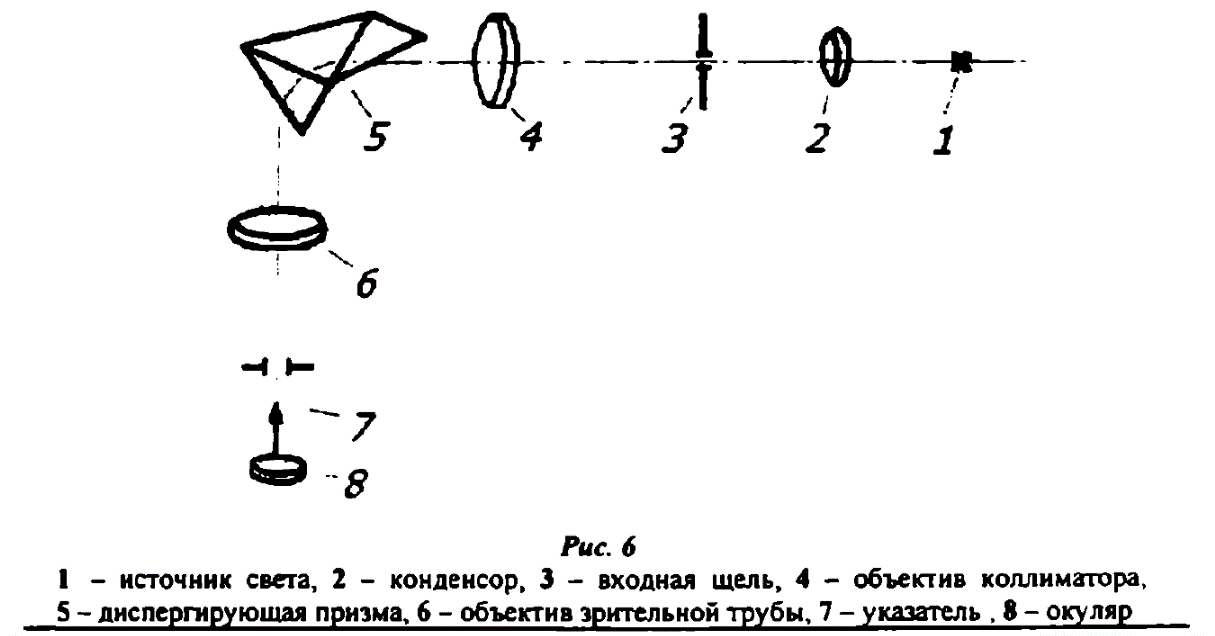
\includegraphics[scale=0.5]{1}%
		}
	
		\vskip 0.5cm
	
		\caption{Оптическая схема системы конденсор / коллиматор}

		\raisebox{-.5\height}{%
			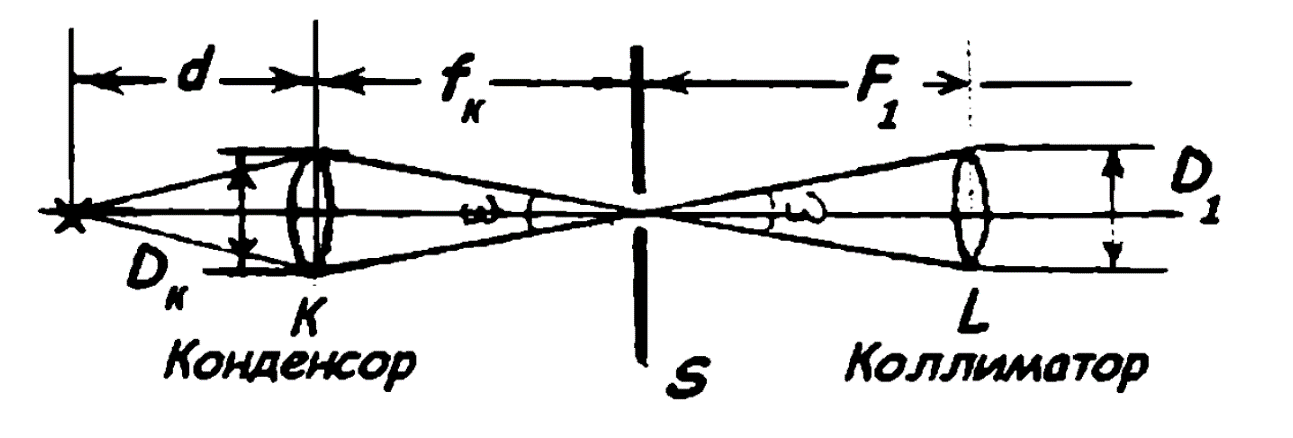
\includegraphics[scale=0.5]{2}%
		}
		
	\end{figure}
	
\end{document}